\chapter{Introducción}

\begin{chapquote}{Miguel de Cervantes, \textit{Don Quijote de la Mancha}}
Sola una cosa tiene mala el sueño, según he oído decir, y es que se parece a la muerte, pues de un dormido a un muerto hay muy poca diferencia.
\end{chapquote}

Viendo el enfoque actual que se le ha dado al problema \sat, y su capacidad para adaptarse a distintos escenarios, motiva a buscar cualquier mejora o aceleramineto en un algoritmo que lo resuelva. Este problema ha sido ampliamente estudiado, siguiendo una misma linea que en el presente ha alcanzado buenas implementaciones de una solución. Aunque, existe la posibilidad de explorar una visión alternativa, y esta permita abrir una puerta a nuevas soluciones.

Muchos problemas pueden expresarse como proposiciones lógicas, como los problemas de satisfacción de restricciones (\textit{CSP}), y eso permite abarcar una area mayor de impacto en el caso de realizar avances científicos cuando se busca una solución a \sat. Actualmente las soluciones están centradas en la forma normal conjuntiva (\textit{CNF}) de una proposición booleana, esto se debe a que permite descartar facilmente una asignación de valores (\textit{TRUE} o \textit{FALSE}) para las variables involucradas en la fórmula lógica. Esta representación separa las proposiciones en cláusulas, si alguna de ellas no se cumple, se puede descartar el resto de ellas. Por otro lado, las implementaciones actuales tienen enfoques diferentes, algunas secuenciales, otras en paralelo y también exiten otras más probabilísticas pero manteniendo la misma representación.

En ciertos casos, se puede ver una representación como los diagramas binarios de desición (\textit{BDDs}) para resolver \sat, esta puede tener ventajas en ciertos aspectos, u ocasiones, pero sigue sin tener el impacto que tiene \textit{CNF}. Hay implementaciones que usan paralelismo para solucionar \sat pero este tipo de estrategias tienden a ser más dificiles de implementar para estructuras arborescentes como los \textit{BDDs}. Por lo tanto, el objetivo es encontrar una representación que pueda brindar un nuevo enfoque a \sat y que tenga la versatilidad para tener implementaciones en paralelo.

El polinomio de \textit{Zhegalkin} es una representación para proposiciones booleanas, basada en los polinomios usuales en algebra, esta traduce los operadores lógicas de conjunción ($\land$), disyunción ($\lor$), implicación ($\implies$), equivalencia ($\iff$) y negación o complemento ($\neg$), a un polinomio que solo posee dos operadores, conjunción ($\cdot$) y disyunción exclusiva ($\oplus$). Una ventaja de esta representación es que solo la existencia de un polinomio para una fórmula lógica implica su satisfactibilidad. Otro aspecto importante es la posibilidad de implementar una solución que opere en paralelo, ya que los polinomios tienen una estructura propicia para separarse en tareas que pueden delegarse.

\section{\textit{CSP}}

Los problemas de satisfacción de restricciones (\textit{CSP}) son preguntas formuladas a partir de un conjunto de objectos cuyo estado está definido por un número finito de limitaciones. Algunos de estos problemas son conocidos, por ejemplo un sudoku, crucigrama, coloración de grafos, el problema de las ocho reinas, entre otros. Todos ellos son traducibles a \sat, un ejemplo de ello se puede ver en las figuras \ref{fig:g_col_csp} y \ref{fig:g_col_sat}, donde se muestra el mismo problema de coloración del grafo en la figura \ref{fig:graph} modelado de forma diferente.

En la figura \ref{fig:g_col_sat} se construye una proposición lógica siguiendo una notación para el nombre de las variables donde la primera letra es el nodo en minúsculas y la segunda es el color, por ejemplo \textit{ar} es el nodo \textit{A} de color rojo. Solo se muestra el nodo \textit{A} pero sigue el mismo patrón para los otros nodos.

\begin{figure}
\centering
\begin{minipage}{0.5\textwidth}
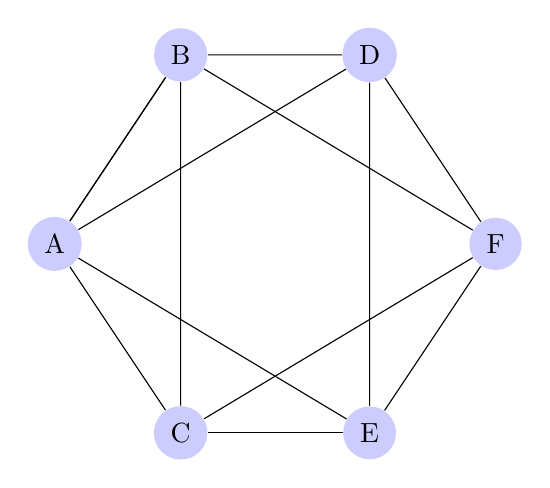
\begin{tikzpicture}
  [scale=.8,auto=left,every node/.style={circle,fill=blue!20}]
  \node (n1) at (2,4) {A};
  \node (n2) at (4,7) {B};
  \node (n3) at (4,1) {C};
  \node (n4) at (7,7) {D};
  \node (n5) at (7,1) {E};
  \node (n6) at (9,4) {F};

  \draw (n1) -- (n2);
  \draw (n1) -- (n2);
  \draw (n1) -- (n3);
  \draw (n1) -- (n4);
  \draw (n1) -- (n5);

  \draw (n2) -- (n3);
  \draw (n2) -- (n4);
  \draw (n2) -- (n6);

  \draw (n3) -- (n5);
  \draw (n3) -- (n6);

  \draw (n4) -- (n5);
  \draw (n4) -- (n6);

  \draw (n5) -- (n6);
\end{tikzpicture}
\caption{Grafo sin colorear}
\label{fig:graph}
\end{minipage}\hfill
\begin{minipage}{0.5\textwidth}
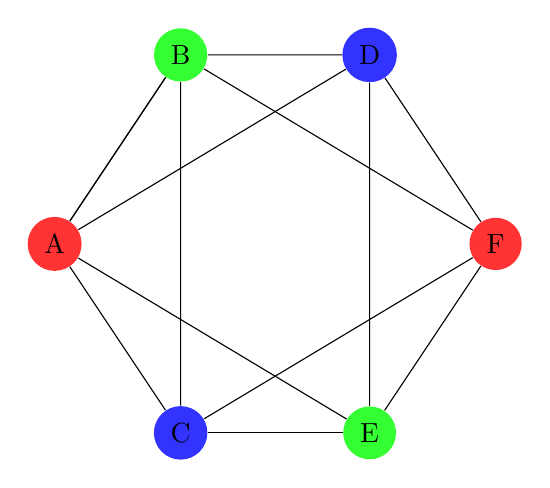
\begin{tikzpicture}
  [scale=.8,auto=left,every node/.style={circle}]
  \node[fill=red!80] (n1) at (2,4) {A};
  \node[fill=green!80] (n2) at (4,7) {B};
  \node[fill=blue!80] (n3) at (4,1) {C};
  \node[fill=blue!80] (n4) at (7,7) {D};
  \node[fill=green!80] (n5) at (7,1) {E};
  \node[fill=red!80] (n6) at (9,4) {F};

  \draw (n1) -- (n2);
  \draw (n1) -- (n2);
  \draw (n1) -- (n3);
  \draw (n1) -- (n4);
  \draw (n1) -- (n5);

  \draw (n2) -- (n3);
  \draw (n2) -- (n4);
  \draw (n2) -- (n6);

  \draw (n3) -- (n5);
  \draw (n3) -- (n6);

  \draw (n4) -- (n5);
  \draw (n4) -- (n6);

  \draw (n5) -- (n6);
\end{tikzpicture}
\caption{Grafo coloreado}
\label{fig:graph_color}
\end{minipage}
\end{figure}

\begin{figure}
\begin{align*}
    & A, B, C, D, E, F \in \{Red,\ Green,\ Blue\}\\
    \\
    & A \neq B \land A \neq C \land A \neq D \land A \neq E\\
    & B \neq C \land B \neq D \land B \neq E \land B \neq F\\
    & C \neq E \land C \neq F\\
    & D \neq E \land D \neq F\\
    & E \neq F
\end{align*}
\caption{Restricciones para la coloración del grafo}
\label{fig:g_col_csp}
\end{figure}

\begin{figure}
\begin{align*}
    (ar \lor ag \lor ab)\ \land\\
    \neg(ar \land ag)\ \land \neg(ar \land ab)\ \land \neg(ag \land ab)\ \land\\
    \neg(ar \land br)\ \land \neg(ar \land cr)\ \land \neg(ar \land dr)\ \land \neg(ar \land er)\ \land\\
    \neg(ag \land bg)\ \land \neg(ag \land cg)\ \land \neg(ag \land dg)\ \land \neg(ag \land eg)\ \land\\
    \neg(ab \land bb)\ \land \neg(ab \land cb)\ \land \neg(ab \land db)\ \land \neg(ab \land eb)\ \land\\
    \vdots
\end{align*}
\caption{Restricciones para la coloración del grafo en \sat}
\label{fig:g_col_sat}
\end{figure}

\section{Estructura del trabajo}

En los siguientes capítulos se describirá el proceso de implementación a una solución a \sat, comenzando por definir detalladamente esta representación junto a las implementaciones que se desarrollaron. Siguiendo con el diseño de una implementación que aproveche los recursos de la \textit{GPU}, a través de la plataforma OpenCL. Es importante resaltar, que para este trabajo trabajo se ha usado la versión \texttt{1.2}; en todo momento que se refiera a esta plataforma, la versión es tácita. También se describen otros soluciones que se implementaron, seguidas de los resultados experimentales obtenidos y un breve análisis de los mismos. Finalizando con las conclusiones y posibles trabajos futuros.
